% !TEX root = ../masterthesis.tex
\chapter{Entangled photon generation using adiabatic rapid passage with frequency-chirped pulses}
\label{cha:chirp}

\section{Introduction and motivation}

In order to efficiently use the biexciton decay cascade the \acl{XX} state has to be prepared beforehand in a robust way.
This chapter deals with the efficient inversion of the \ac{QD} from the ground state to the biexciton level via \ac{ARP}.
\acs{ARP} uses chirped pulses, which need to be measured and deterministically adjusted in order to effectively use them.
Therefore, the majority of this chapter will focus on the chirp and how to determine and adjust it, with the help of simulations and later with measurements.
 

\section{Chirp}
\label{sec:chirp}
A chirped signal is a signal of which the frequency changes over time.
For example, the frequency of a linearly chirped signal $f(t)$ would be described by
\begin{equation}
f(t) = ct+f_0
\end{equation}
where $f_0$ is the starting frequency at $t=0$ and $c$ is the chirpyness. A linear chirped sinusoidal wave is depicted in figure~\ref{fig:chirped-sin}.

\begin{figure}[H]
	\centering
	\includegraphics[width=\linewidth]{figures/chirp/plots/chirped-sin}
	\caption{A chirped sinusoidal wave which increases in frequency over time.}
	\label{fig:chirped-sin}
\end{figure}

As this chapter is concentrated on exciting \acp{QD} with frequency-chirped pulses, the mathematical description of chirped laser pulses will now be discussed. The electric field of a laser $E(t)$ has the shape
\begin{equation}
\label{eq:electric-field-laser}
E(t) \sim \mathrm{Re}\left(f^{1/2}(t) \cdot \exp\left(-i \omega t - i \phi(t)\right)\right)
\end{equation}
with the central frequency $\omega$ and the linear chirp $\phi(t)$.

Depending on the laser either a Gaussian or a hyperbolic secant describes the pulse shape more accurately~\cite{glassl_biexciton_2013, hirayama_real-time_2002}

\begin{itemize}
	\item Gaussian pulse:
	\begin{itemize}
		\item Pulse shape of
		\begin{equation}
		\label{eq:f_gauss}
		f_{gauss}(t) = \left(\frac{A_{gauss}}{\sqrt{2 \cdot \pi \cdot \tau_0 \cdot \tau}} \exp\left(-\frac{t^2}{2 \cdot \tau^2}\right)\right)^2
		\end{equation}
		with the normalization constant $A_{gauss}$, the pulse duration $\tau_0$, the central frequency $\omega$ and the chirp coefficient $\alpha$.
		\item Linear chirp of
		\begin{equation}
		\label{eq:phi-gauss}
		\phi_{gauss}(t) = \frac{a_{gauss} t^2}{2}
		\end{equation}
		where $\tau = \sqrt{\alpha^2 / \tau_0^2 + \tau_0^2}$ characterizes the chirped pulse length and $a = \alpha / (\alpha ^ 2 + \tau _0 ^ 4)$ is the frequency chirp rate.
	\end{itemize}
	\item Secant pulse:
	\begin{itemize}
		\item Pulse shape of
		\begin{equation}
		f_{secant}(t) = A_{secant} \cdot sech^2\left(\frac{t}{\tau_0}\right) = A_{secant} \cdot \left(\frac{2}{exp(\frac{t}{\tau_0}) + exp(-\frac{t}{\tau_0})}\right)^2
		\end{equation}
		with the normalization constant $A_{secant}$, the pulse duration $\tau_0$, the central frequency $\omega$ and the chirp coefficient $\alpha$.
		\item Linear chirp of
		\begin{equation}
		\phi_{secant}(t) = \alpha_{secant}\left(\frac{t}{\tau_0}\right)^2
		\end{equation}
	\end{itemize}
\end{itemize}
	
The following discussion in this chapter will assume laser pulses with a Gaussian shape. 


\section{Measuring the chirp with interferometric autocorrelation}

In order to estimate the pulse width $\tau_0$ \ac{IAC} is used.
Basically, a nonlinear crystal is added to a Michelson interferometer in order to generate a signal governed by
\begin{equation}
\label{eq:i-m-integral}
I_M(\tau) = \int_{-\infty}^{+\infty}\langle|(E(t)+E(t-\tau))^2|^2\rangle dt.
\end{equation}
Here $\langle \rangle$ denotes averaging over fast oscillations of the electric field and the integral stands for integration over the pulse envelope.
Under the use of equation~\ref{eq:electric-field-laser} it can be expanded to
\begin{align}
I_M(\tau) = 1 &+ 2 \int f(t) f(t + \tau) dt + \int f(t) f(t + \tau) cos(2 \omega \tau + 2 \Delta \phi) dt \nonumber\\
&+ 2 \int f^{1/2}(t) f^{3/2}(t + \tau) cos(\omega \tau + \Delta \phi) dt + 2 \int f^{3/2}(t) f^{2/2}(t + \tau) cos(\omega \tau + \Delta \phi) dt
\end{align}
where $\Delta \phi(t, \tau) = \phi(t + \tau) - \phi(t)$ and $\int f(t) dt = 1$.
\begin{figure}[H]
	\centering
	\includegraphics[width=0.8\linewidth]{figures/chirp/Optical-interferometric-autocorrelation-setup.png}
	\caption[Schematics of an interferometric autocorrelator]{Schematics of an interferometric autocorrelator, where \textbf{L} is a converging lens, \textbf{SHG} a second-harmonic generation crystal, \textbf{BS} a beam splitter and \textbf{F} a spectral filter to block the fundamental wavelength~\cite{noauthor_optical_nodate}.}
	\label{fig:optical-field-autocorrelation-setup}
\end{figure}
As will be shown in section~\ref{sec:fabry-simulation} the chirp parameter $\alpha$ has hardly any measurable influence on the resulting signal. However, certain modifications to the \ac{IAC} signal introduced by \textcite{hirayama_real-time_2002} makes it much more sensitive to the temporal chirp.
It is called \ac{MOSAIC} and it performs the following transformations on the \ac{IAC} spectrum: the $\omega$ terms are eliminated and the $2\omega$ term is doubled.
The \ac{MOSAIC} signal is then described by the following equation
\begin{equation}
\label{eq:i-m-filtered}
I_{M, filtered}(\tau) = 1 + 2 \int f(t) f(t + \tau) dt + 2 \int f(t) f(t + \tau) cos(2\omega \tau + 2\Delta \phi) dt
\end{equation}

\section{Deterministically adjusting the chirp with a pulse expander}
\label{sec:pulse-expander}
In the optimal case the chirp of the pulse can be deterministically adjusted in order to most efficiently excite the \ac{QD} via adiabatic rapid passage described in section~\ref{sec:arp}.
Grating compressors as discussed by \textcite{martinez_3000_1987} were originally used to compensate the broadening of fibers.
However, together with a telescope they have the inverse effect and can be used to induce a positive chirp. 
A setup like this sketched in figure~\ref{fig:pulse-expander} can be used to will in future references in this work be called \textit{pulse expander}.
The accumulated group velocity dispersion, linked to the chirp, is described by
\begin{equation}
\frac{d^2 \Phi}{d \omega^2} = k \beta^2 2 z
\end{equation}
where $z$ is the (adjustable) distance between the grating and focal plane of the lens and $\beta$ depends on the parameters of the grating and the lens.

\begin{figure}[H]
	\centering
	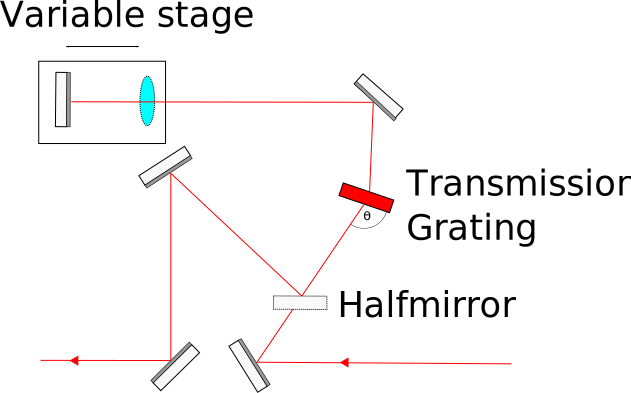
\includegraphics[width=0.7\linewidth]{figures/chirp/pulse-expander}
	\caption{Scheme of a folded pulse expander as described by \textcite{martinez_3000_1987}}
	\label{fig:pulse-expander}
\end{figure}

\section{Adiabatic rapid passage}
\label{sec:arp}
One way to inverse the \ac{QD} from the ground state to the biexciton state is by exciting it with a transform-limited laser pulse of constant center frequency, which is equals to half of the ground state biexciton transition frequency.
However, in order to ensure the inversion precise control of the field intensity is required~\cite{glassl_biexciton_2013}.
Adiabatic rapid passage \acused{ARP} (\acs{ARP}) with frequency chirped is an alternative to this Rabi-flopping scheme.
Basically, the goal is to adiabatically excitee from ground state to biexciton state without energy-level crossing~\cite{hui_proposal_2008}.
Schemes which provide that, are also stable with respect to intensity changes of the laser field.

In order to calculate the final biexciton occupation, \textcite{glassl_biexciton_2013} assumed linearly-chirped Gaussian laser pulse as discussed in section~\ref{sec:chirp}.
The simulation results are visible in figure~\ref{fig:biexciton-occupation}.
\begin{figure}[H]
	\centering
	\includegraphics[width=\linewidth]{figures/chirp/biexciton-occupation}
	\caption{Final biexciton occupation after chirped Gaussian pulse of pulse duration $\tau_0 = \SI{2}{\pico \second}$.
		It is plotted vertically as a function of the original pulse area $A$ and vertically as a function of the chirp $\alpha$ for biexciton binding energies of (a) $\Delta=0$, (b) 1, and (c) \SI{3}{\milli \electronvolt}~\cite{glassl_biexciton_2013}.}
	\label{fig:biexciton-occupation}
\end{figure}
The central frequency is chosen so that for $\alpha=0$ it resonates to ground state biexction transition, which is sketched in figure~\ref{fig:biexciton-occupation}.
For $\alpha=0$ Rabi oscillations are visible and its period depends strongly on the biexciton binding energy $\Delta$.
However, for $\alpha \gg 0$ biexciton preparation becomes insensitive to small variations to the pulse area $A$ as long it exceeds a certain threshold.
This is therefore the regime which would be the most suitable to work in.
In the case of $\alpha < 0$ this fails for moderate values of $\Delta$ as can be seen in figure~\ref{fig:biexciton-occupation}(b).


\section{Simulation}
\label{sec:fabry-simulation}
The electric field $E$ of a chirped laser pulse is described by equation~\eqref{eq:electric-field-laser}.
The following discussion will assume a Gaussian laser shape as described by equation~\eqref{eq:f_gauss} and \eqref{eq:phi-gauss}.
A simulation for $E$ is plotted for different chirp parameters $\alpha$  in figure~\ref{fig:chirpedlaserpulse}.
The chirp parameter strongly influences the shape of the electric field and could be estimated if $E$ could be measured directly which is unfortunately not the case.

\begin{figure}[H]
	\centering
	\includegraphics[width=\linewidth]{figures/chirp/plots/chirped_laser_pulse}
	\caption{Electric field $E$ of Gaussian laser pulse of pulse duration $\tau_0=\SI{0.5}{\pico \second}$ for chirp of (a) $\alpha = \SI{0}{\pico \second \squared}$ and (b) $\alpha = \SI{0.5}{\pico \second \squared}$}
	\label{fig:chirpedlaserpulse}
\end{figure}

However, the laser signal can be sent into an \ac{IAC} which outputs a signal as shown in figure~\ref{fig:imgausschirpwithoutslitwithoutmosaic} and described by equation~\eqref{eq:i-m-integral}.
However, the chirp only marginally influences the resulting signal.

\begin{figure}[H]
	\centering
	\includegraphics[width=\linewidth]{figures/chirp/plots/I_M_gauss_chirp_without_slit_without_MOSAIC}
	\caption{Intensity of IAC of a Gaussian laser pulse of pulse duration $\tau_0=\SI{0.5}{\pico \second}$ with applied MOSAIC filter for chirp of (a) $\alpha = \SI{0}{\pico \second \squared}$ and (b) $\alpha = \SI{0.5}{\pico \second \squared}$}
	\label{fig:imgausschirpwithoutslitwithoutmosaic}
\end{figure}

That is why the MOSAIC filter is applied which results in a signal as shown in figure~\ref{fig:mosaicchirpedlaserpulse} and described by equation~\eqref{eq:i-m-filtered}.
Now the influence of the chirp is clearly visible in the lower envelope.

\begin{figure}[H]
	\centering
	\includegraphics[width=\linewidth]{figures/chirp/plots/mosaic_chirped_laser_pulse}
	\caption{Intensity of IAC of a Gaussian laser pulse of pulse duration $\tau_0=\SI{0.5}{\pico \second}$ with applied MOSAIC filter for chirp of (a) $\alpha = \SI{0}{\pico \second \squared}$ and (b) $\alpha = \SI{0.5}{\pico \second \squared}$}
	\label{fig:mosaicchirpedlaserpulse}
\end{figure}

The points of the lower envelope can be obtained by determining the local minima of the signal as shown in figure~\ref{fig:mosaicchirpedlaserpulsefindenvelope}.

\begin{figure}[H]
	\centering
	\includegraphics[width=\linewidth]{figures/chirp/plots/mosaic_chirped_laser_pulse_find_envelope}
	\caption{Intensity of IAC of a Gaussian laser pulse of pulse duration $\tau_0=\SI{0.5}{\pico \second}$ with applied MOSAIC filter for chirp of (a) $\alpha = \SI{0}{\pico \second \squared}$ and (b) $\alpha = \SI{0.5}{\pico \second \squared}$.
	The orange dots are results of a numerical peak finder algorithm, executed in order to find local minima.}
	\label{fig:mosaicchirpedlaserpulsefindenvelope}
\end{figure}

The lower bound (minima envelope) of the MOSAIC trace can be derived by use of the standard textbook procedure~\cite{klein_optics_1986}
\begin{equation}
S^{min}_{MOSAIC}(\tau)= 1 + 2 \cdot g(\tau) - 2 \cdot [g_s^2(\tau)+g_c^2(\tau)]^{1/2}
\end{equation}
with 
\begin{align}
g(\tau)&=\int f(t)f(t+\tau)dt\\
g_s(\tau)&=\int f(t)f(t+\tau)sin(2\Delta\phi)dt\\
g_c(\tau)&=\int f(t)f(t+\tau)cos(2\Delta\phi)dt
\end{align}
The points of the lower envelope determined before can now be fitted in order to obtain the chirp parameter $\alpha$ as shown in figure~\ref{fig:mosaicchirpedlaserpulsefitenvelope}.
It is visible that the fitted values of $\alpha$ correspond to the expected values.
\begin{figure}[H]
	\centering
	\includegraphics[width=\linewidth]{figures/chirp/plots/mosaic_chirped_laser_pulse_fit_envelope}
	\caption[Intensity of IAC of a Gaussian laser pulse of pulse duration $\tau_0=\SI{0.5}{\pico \second}$ with applied MOSAIC filter and fitted $\alpha$-values.]{Intensity of IAC of a Gaussian laser pulse of pulse duration $\tau_0=\SI{0.5}{\pico \second}$ with applied MOSAIC filter for chirp of (a) $\alpha = \SI{0}{\pico \second \squared}$ and (b) $\alpha = \SI{0.5}{\pico \second \squared}$.
	The orange line is a fit for the lower envelope of the MOSAIC signal in order to obtain $\alpha$.}
	\label{fig:mosaicchirpedlaserpulsefitenvelope}
\end{figure}

\section{Measurements and discussion}

In order to determine the chirp of a laser pulse which only passed the pulse shaper as shown in figure~\ref{fig:setupflat}, it is sent to the \ac{IAC}.
Afterwards, a signal was measured where an additional pulse expander was inserted as discussed in section~\ref{sec:pulse-expander}.
The comparison between these two is shown in figure~\ref{fig:measuredchirpedlaserpulsebeforemosaic}.
Compared to the simulations in figure~\ref{fig:imgausschirpwithoutslitwithoutmosaic} it is visible, that the IAC of the laser pulse without the pulse expander fits the expected shape well, while the one with the pulse expander does not.
Possible reasons could be that the chirp is too high for the model used in the simulation to work or that the pulse expander introduces side effects not considered in the simulation.

\begin{figure}[H]
	\centering
	\includegraphics[width=\linewidth]{figures/chirp/plots/measured_chirped_laser_pulse_before_MOSAIC}
	\caption{Measured IAC of Ti:Sa Laser without (a) and with (b) pulse expander before the autocorrelator.}
	\label{fig:measuredchirpedlaserpulsebeforemosaic}
\end{figure}

The same signals after applying the \ac{MOSAIC} filter are shown in figure~\ref{fig:measuredchirpedlaserpulseaftermosaic}.
It is visible that the lower envelopes in figure~\ref{fig:measuredchirpedlaserpulseaftermosaic}(a) and (b) do not resemble the expected ones in figure~\ref{fig:mosaicchirpedlaserpulse}.
As laser signals without pulse expander were assumed to be relatively unchirped it is already unexpected that the lower envelope differs that much from a constant line at zero intensity.
One explanatory approach could be that the laser was already chirped to begin with, however this would not explain why the shape of the lower envelope differs from the characteristic one of the simulation.

\begin{figure}[H]
	\centering
	\includegraphics[width=\linewidth]{figures/chirp/plots/measured_chirped_laser_pulse_after_MOSAIC}
	\caption{Measured IAC of Ti:Sa Laser with applied MOSAIC filter without (a) and with (b) pulse expander before the autocorrelator.}
	\label{fig:measuredchirpedlaserpulseaftermosaic}
\end{figure}


